\chapter{Что ты такое?}
\label{ch:chap5}
Параметры системы:
$$
    R_1 = 7083, \tab R_2 = 14165, \tab C = 277\mu F
$$
\begin{itemize}
    \item $R_1$  - сопротивление входного резистора
    \item $R_2$  - сопротивление отрицательной обратной связи
    \item $C$  - ёмкость конденсатора отрицательной обратной связи
\end{itemize}

\begin{figure}[ht]
  \centering
  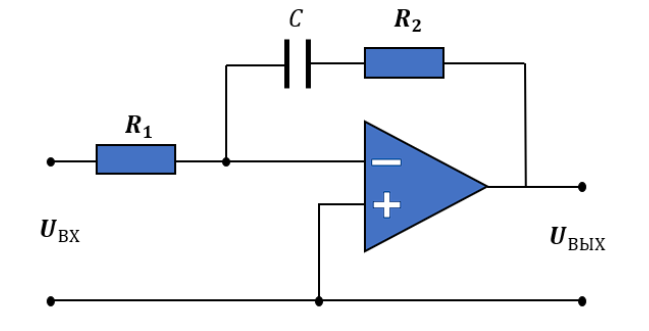
\includegraphics[width=0.8\textwidth]{op_ampl.png}
  \caption{Принципиальная схема регулятора на операционном усилителе}
\end{figure}

Входом объекта считается $U_{in}(t)$, а выходом $U_{out}(t)$. 

\section{Передаточная функция}
\href{https://gg0715.narod.ru/esa/13.html}{Как можно заметить}, на обратной связи у нас есть конденсатор, который можно интерпретировать как И компоненту регулятора, а операционный усилитель как П компоненту, который контролируется его резистором $R_2$. Получаем ПИ-регулятор.
Ему соответствуется изодромное звено - интегрирующее + форсирующее звенья.
$$
W_{I}(s) = \frac{1}{R_1 Cs} = \frac{1}{Ts}
$$
$$
W_{P}(s) = \frac{R_2}{R_1} = k_p
$$
$$
W_{PI}(s) = W_P(s) + W_I(s) = \frac{R_2}{R_1} + \frac{1}{R_1 Cs} = \frac{CR_2 s + 1}{R_1Cs}
$$
Для сокращения записи введём константы $T_1, T_2$ - дифференциальная и интегральная компонента:
$$
W_{PI}(s) = \frac{T_1s + 1}{T_2 s}
$$

\section{Временные  характеристики}
$$
y_{i.r.}(t) = \mathcal{L}^{-1}\{ \frac{T_1s + 1}{T_2 s}  \} = \mathcal{L}^{-1}\{ \frac{T_1}{T_2}\} + \mathcal{L}^{-1}\{ \frac{1}{T_2}\} = \delta (t)\frac{T_1}{T_2} + \frac{1}{T_2}
$$
$$
y_{s.r.}(t) =  \mathcal{L}^{-1}\{ \frac{T_1s + 1}{T_2 s^2} \} = \mathcal{L}^{-1}\{ \frac{T_1}{T_2 s}\} + \mathcal{L}^{-1}\{ \frac{1}{T_2 s^2}\} = \frac{T_1}{T_2} + \frac{t}{T_2}
$$


\begin{figure}[ht]
  \centering
  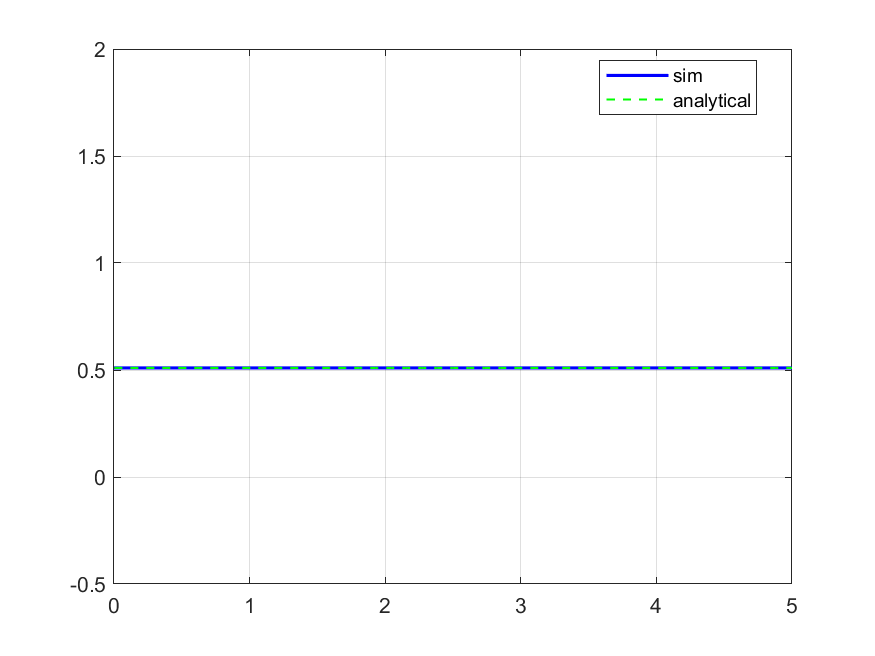
\includegraphics[width=0.8\textwidth]{impulse_responce5.png}
  \caption{Воздействие - \textrm{impulse responce}}
\end{figure}
\newpage
\begin{figure}[ht]
    \centering
    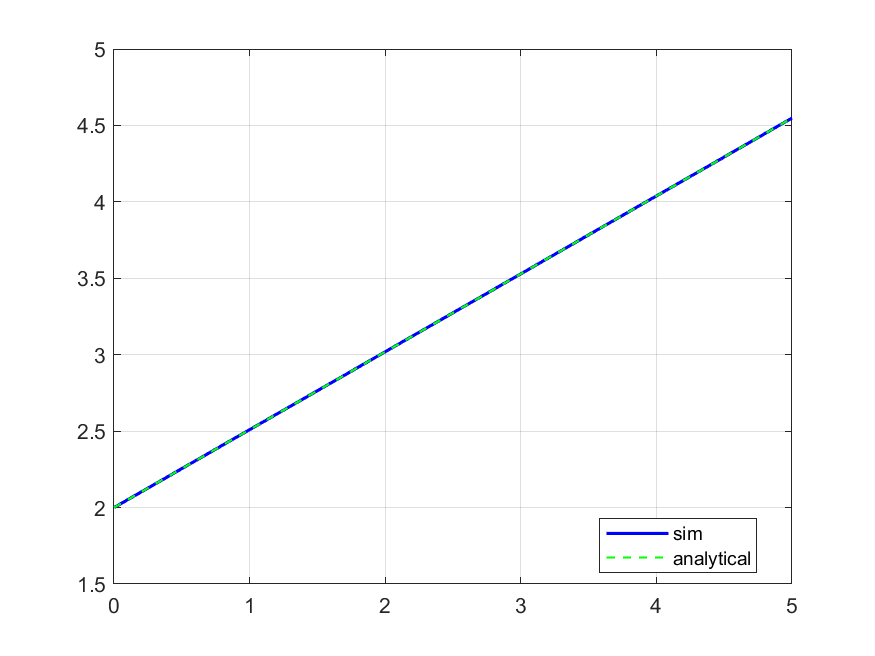
\includegraphics[width=0.8\textwidth]{step_responce5.png}
    \caption{Воздействие - \textrm{step responce}}
  \end{figure}
\newpage

\section{Частотные характеристики}
$$
W(j\omega) =  \frac{T_1 j\omega + 1}{T_2 j \omega} = \frac{T_1}{T_2} + \frac{1}{T_2j\omega} = \frac{T_1}{T_2} - j\frac{1}{T_2\omega}
$$
Амплитудно-частотная характеристика:
$$
A(\omega) = \sqrt{P^2 + Q^2} = \sqrt{(\frac{T_1}{T_2})^2 + (\frac{1}{T_2\omega})^2}
$$
Логарифмическая-Амплитудно-частотная характеристика:
$$
L(\omega) = 20lg(A) = 10lg( (\frac{T_1}{T_2})^2 + (\frac{1}{T_2\omega})^2 )
$$
Фазовая-частотная характеристика:
$$
\phi(\omega) = atan2(Q,P) = -atan2(\frac{1}{T_2\omega} , \frac{T_1}{T_2})
$$
\newpage
\begin{figure}[ht]
  \centering
  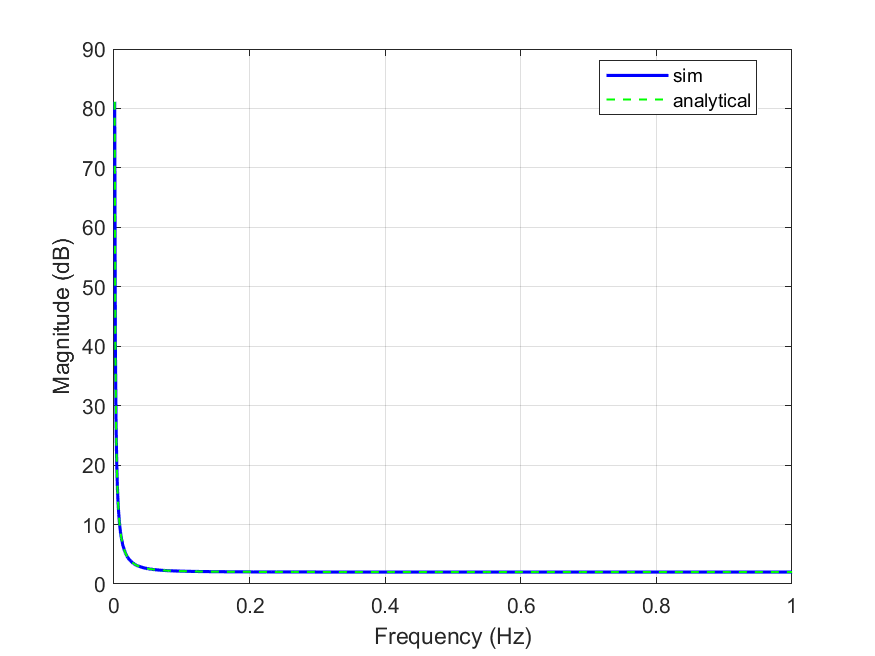
\includegraphics[width=0.8\textwidth]{freq_ampl5.png}
\caption{Сравнение - АЧХ}
\end{figure}

\begin{figure}[ht]
    \centering
    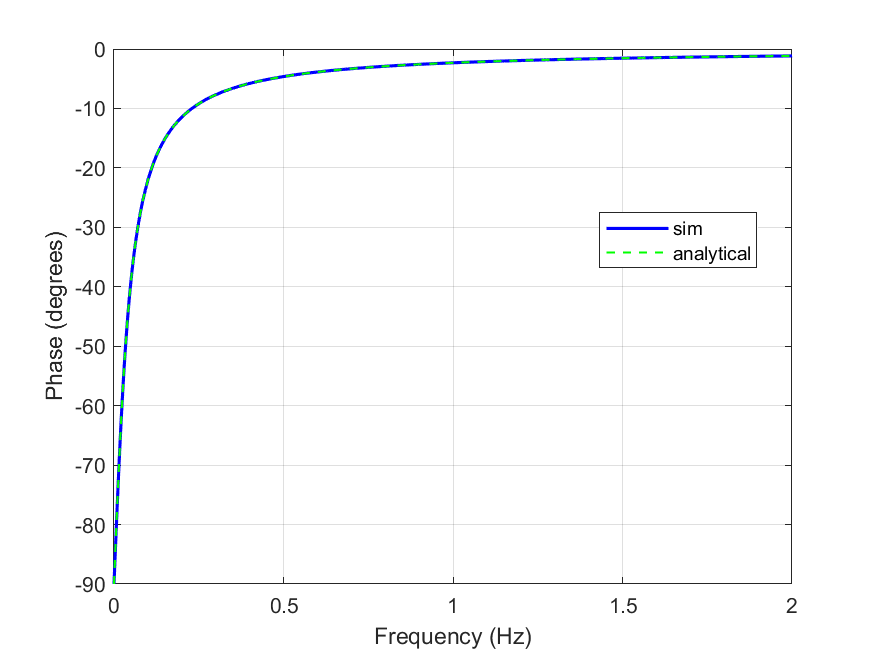
\includegraphics[width=0.8\textwidth]{freq_phase5.png}
  \caption{Сравнение - ФЧХ}
  \end{figure}
\newpage
\begin{figure}[ht]
    \centering
    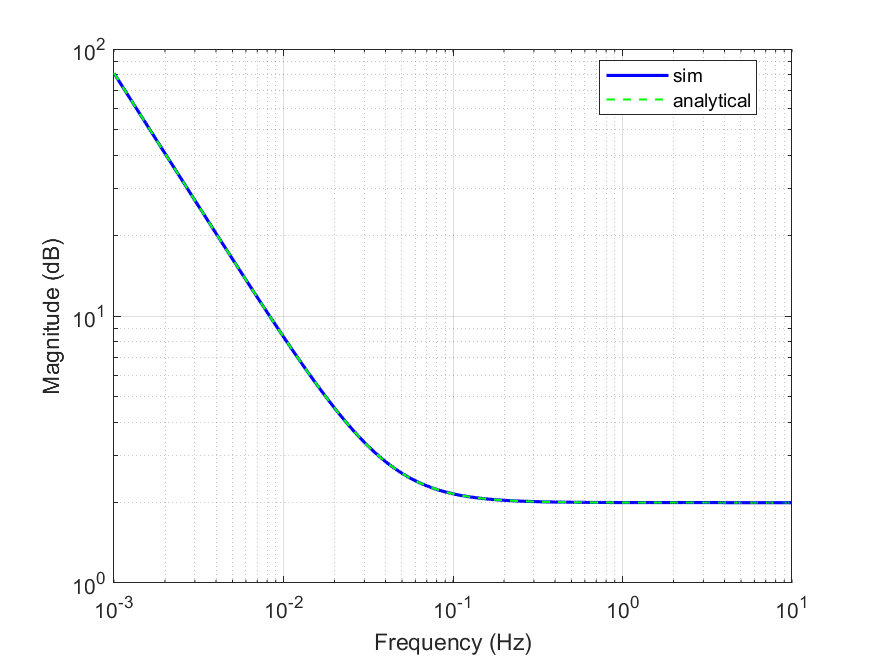
\includegraphics[width=0.8\textwidth]{lfreq_ampl5.png}
  \caption{Сравнение - ЛАЧХ}
  \end{figure}
  
  \begin{figure}[ht]
      \centering
      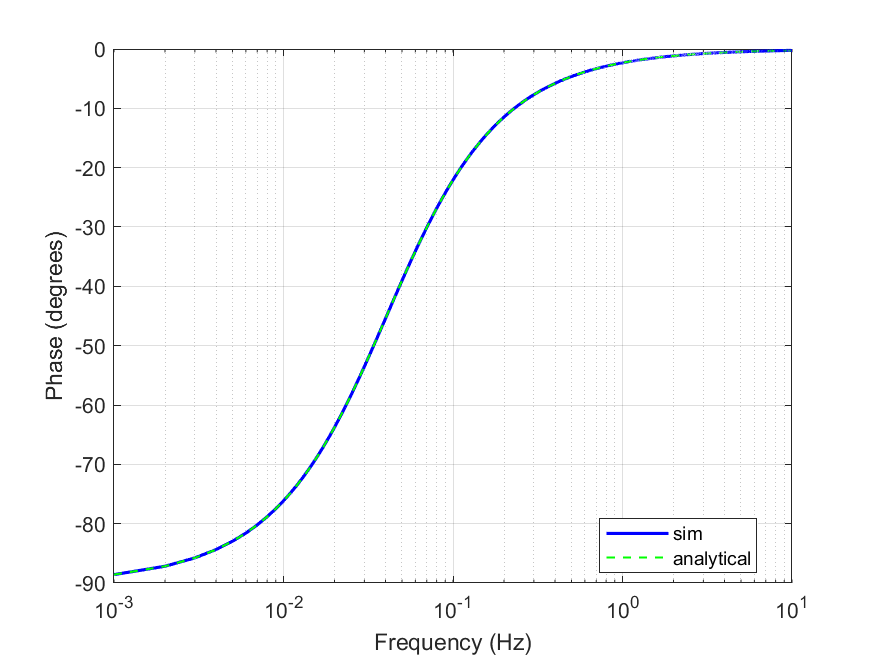
\includegraphics[width=0.8\textwidth]{lfreq_phase5.png}
    \caption{Сравнение - ЛФЧХ}
    \end{figure}

    % \begin{figure}[ht]
    %   \centering
    %   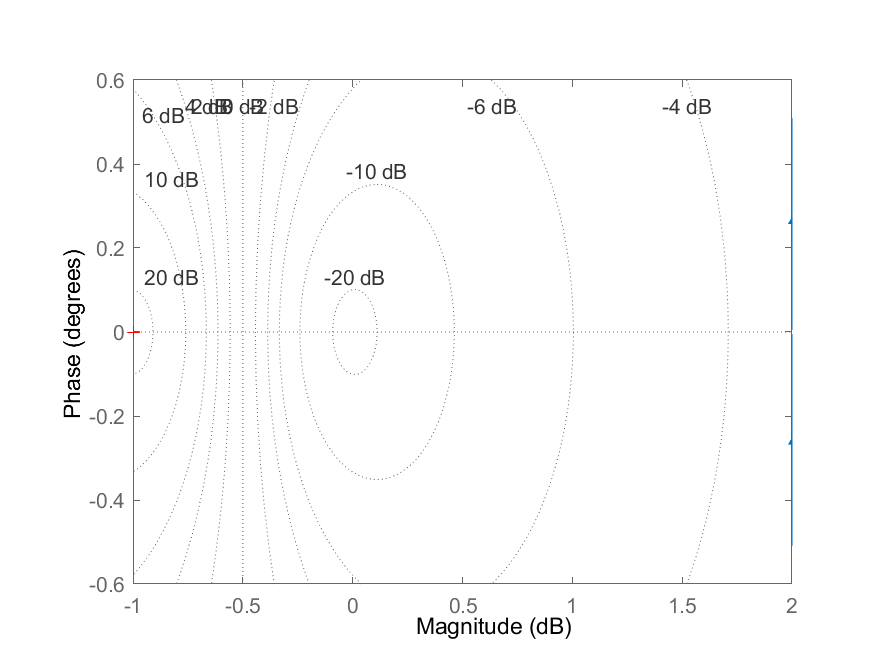
\includegraphics[width=0.8\textwidth]{nyquist5.png}
    % \caption{АФЧХ}
    % \end{figure}
\newpage

\endinput